\documentclass[bachelor, och, labwork]{shiza}
% параметр - тип обучения - одно из значений:
%    spec     - специальность
%    bachelor - бакалавриат (по умолчанию)
%    master   - магистратура
% параметр - форма обучения - одно из значений:
%    och   - очное (по умолчанию)
%    zaoch - заочное
% параметр - тип работы - одно из значений:
%    referat    - реферат
%    coursework - курсовая работа (по умолчанию)
%    diploma    - дипломная работа
%    pract      - отчет по практике
% параметр - включение шрифта
%    times    - включение шрифта Times New Roman (если установлен)
%               по умолчанию выключен
\usepackage{subfigure}
\usepackage{tikz,pgfplots}
\pgfplotsset{compat=1.5}
\usepackage{float}

%\usepackage{titlesec}
\setcounter{secnumdepth}{4}
%\titleformat{\paragraph}
%{\normalfont\normalsize}{\theparagraph}{1em}{}
%\titlespacing*{\paragraph}
%{35.5pt}{3.25ex plus 1ex minus .2ex}{1.5ex plus .2ex}

\titleformat{\paragraph}[block]
{\hspace{1.25cm}\normalfont}
{\theparagraph}{1ex}{}
\titlespacing{\paragraph}
{0cm}{2ex plus 1ex minus .2ex}{.4ex plus.2ex}

% --------------------------------------------------------------------------%


\usepackage[T2A]{fontenc}
\usepackage[utf8]{inputenc}
\usepackage{graphicx}
\graphicspath{ {./images/} }
\usepackage{tempora}

\usepackage[sort,compress]{cite}
\usepackage{amsmath}
\usepackage{amssymb}
\usepackage{amsthm}
\usepackage{fancyvrb}
\usepackage{listings}
\usepackage{listingsutf8}
\usepackage{longtable}
\usepackage{array}
\usepackage[english,russian]{babel}

% \usepackage[colorlinks=true]{hyperref}
\usepackage{url}

\usepackage{underscore}
\usepackage{setspace}
\usepackage{indentfirst} 
\usepackage{mathtools}
\usepackage{amsfonts}
\usepackage{enumitem}
\usepackage{tikz}

\newcommand{\eqdef}{\stackrel {\rm def}{=}}
\newcommand{\specialcell}[2][c]{%
\begin{tabular}[#1]{@{}c@{}}#2\end{tabular}}

\renewcommand\theFancyVerbLine{\small\arabic{FancyVerbLine}}

\newtheorem{lem}{Лемма}

\begin{document}

% Кафедра (в родительном падеже)
\chair{}

% Тема работы
\title{Фрагментация сетей}

% Курс
\course{2}

% Группа
\group{231}

% Факультет (в родительном падеже) (по умолчанию "факультета КНиИТ")
\department{факультета КНиИТ}

% Специальность/направление код - наименование
%\napravlenie{09.03.04 "--- Программная инженерия}
%\napravlenie{010500 "--- Математическое обеспечение и администрирование информационных систем}
%\napravlenie{230100 "--- Информатика и вычислительная техника}
%\napravlenie{231000 "--- Программная инженерия}
\napravlenie{100501 "--- Компьютерная безопасность}

% Для студентки. Для работы студента следующая команда не нужна.
% \studenttitle{Студентки}

% Фамилия, имя, отчество в родительном падеже
\author{Окунькова Сергея Викторовича}

% Заведующий кафедрой
% \chtitle{} % степень, звание
% \chname{}

%Научный руководитель (для реферата преподаватель проверяющий работу)
\satitle{ассистент} %должность, степень, звание
\saname{А. А. Фомин}

% Руководитель практики от организации (только для практики,
% для остальных типов работ не используется)
% \patitle{к.ф.-м.н.}
% \paname{С.~В.~Миронов}

% Семестр (только для практики, для остальных
% типов работ не используется)
%\term{8}

% Наименование практики (только для практики, для остальных
% типов работ не используется)
%\practtype{преддипломная}

% Продолжительность практики (количество недель) (только для практики,
% для остальных типов работ не используется)
%\duration{4}

% Даты начала и окончания практики (только для практики, для остальных
% типов работ не используется)
%\practStart{30.04.2019}
%\practFinish{27.05.2019}

% Год выполнения отчета
\date{2021}

\maketitle

% Включение нумерации рисунков, формул и таблиц по разделам
% (по умолчанию - нумерация сквозная)
% (допускается оба вида нумерации)
% \secNumbering

%-------------------------------------------------------------------------------------------


\begin{enumerate}

    \item Составить и заполнить адресную таблицу.
        
    \begin{figure}[H]
        \centering      %размер рисунка       здесь находится название файла рисунка, без указания формата
        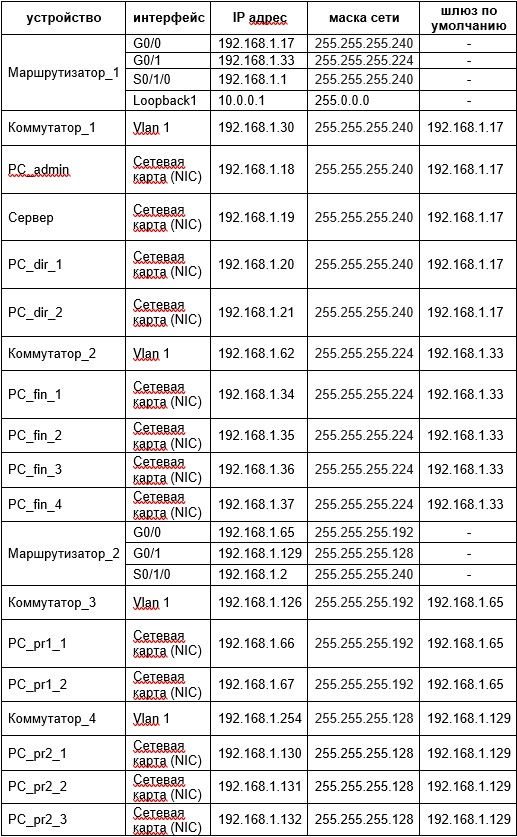
\includegraphics[width=0.75\textwidth]{1}
        \caption{Таблица IP адрессов устройств в заданной конфигурации}
        \label{fig:image1}
    \end{figure}

    \item Запустите Packet Tracer и воспроизведите физическую конфигурацию. Воспользуйтесь для этого 
    результатами предыдущей работы.

    \begin{figure}[H]
        \centering      %размер рисунка       здесь находится название файла рисунка, без указания формата
        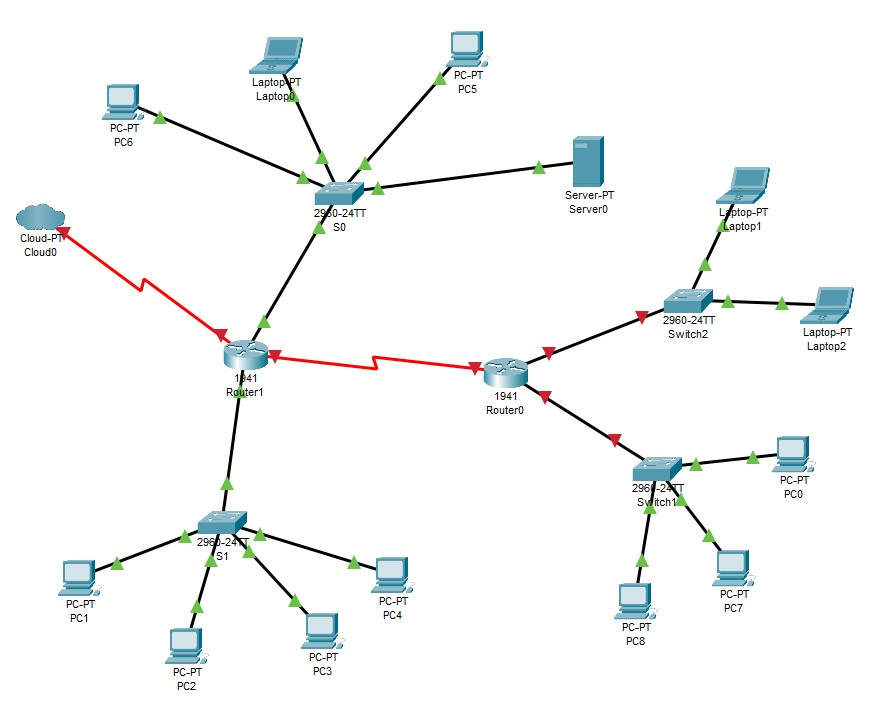
\includegraphics[width=0.75\textwidth]{2}
        \caption{Заданная конфигурация}
        \label{fig:image1}
    \end{figure}

    \item С помощью компьютера администратора и консольного подключения выполните базовое конфигурирование маршрутизаторов:
    
    - задайте уникальные имена
    
    - задайте пароли на консольное подключение
    
    - задайте пароли на доступ к привилегированному пользовательскому режиму
    
    - установите уведомление MOTD, сообщающее о недопустимости несанкционированного доступа к маршрутизаторам
    
    - установите пароли доступа на линии виртуальных терминалов и проверьте их действие
    
    - назначьте IP адреса Ethernet интерфейсам и включите их
    
    - назначьте IP адреса последовательным интерфейсам и включите их
    
    - сохраните конфигурацию
    
    - отключите консольный кабель

    \item С помощью компьютера администратора и консольного подключения внесите необходимые изменения в конфигурации коммутаторов.
    
    \item Внесите необходимые изменения в настройки IPv4 на рабочих станциях, сервере и компьютере администратора.
    
    \item Проверьте доступность с компьютера администратора всех рабочих станций собственной подсети и сервера.
    
    \begin{figure}[H]
        \centering      %размер рисунка       здесь находится название файла рисунка, без указания формата
        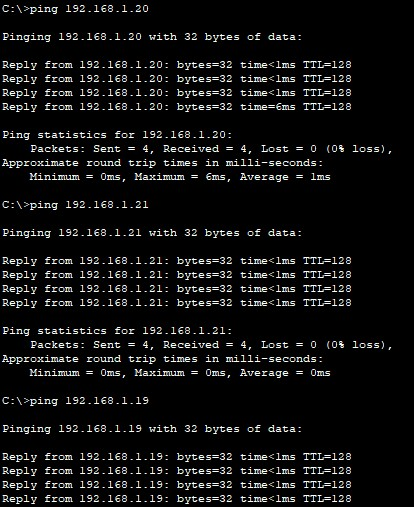
\includegraphics[width=0.75\textwidth]{3}
        \caption{Проверка доступности с компьютера администратора всех рабочих станций собственной подсети и сервера}
        \label{fig:image1}
    \end{figure}

    \item Проверьте доступность с компьютера администратора коммутатора, расположенного в его собственной подсети.
    
    \begin{figure}[H]
        \centering      %размер рисунка       здесь находится название файла рисунка, без указания формата
        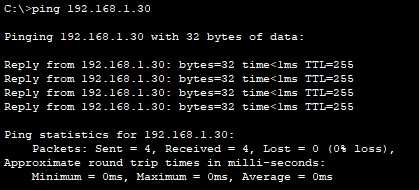
\includegraphics[width=0.75\textwidth]{4}
        \caption{Проверка доступности с компьютера администратора коммутатора, расположенного в его собственной подсети}
        \label{fig:image1}
    \end{figure}

    \item Проверьте доступность с компьютера администратора порта маршрутизатора, расположенного в его собственной подсети.
    
    \begin{figure}[H]
        \centering      %размер рисунка       здесь находится название файла рисунка, без указания формата
        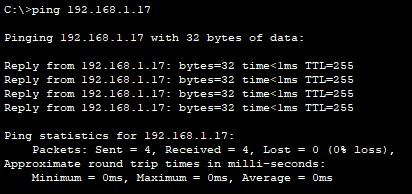
\includegraphics[width=0.75\textwidth]{5}
        \caption{Проверка доступности с компьютера администратора порта маршрутизатора, расположенного в его собственной подсети}
        \label{fig:image1}
    \end{figure}

    \item Проверьте доступность с компьютера администратора остальных портов Маршрутизатора_1.
    
    \begin{figure}[H]
        \centering      %размер рисунка       здесь находится название файла рисунка, без указания формата
        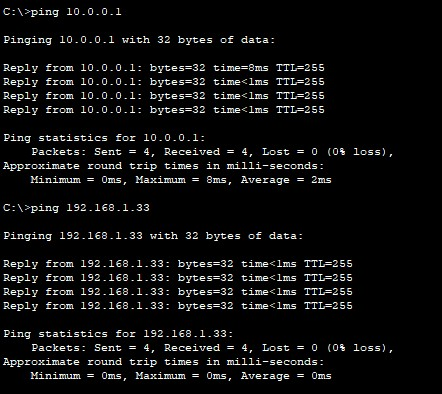
\includegraphics[width=0.75\textwidth]{6}
        \caption{Проверка доступности с компьютера администратора остальных портов Маршрутизатора_1}
        \label{fig:image1}
    \end{figure}

    \item Проверьте доступность с компьютера администратора последовательного порта Маршрутизатора_2.
    
    Для перессылки пакетов с одного маршрутизатора на другой включим протокол rip.

    \begin{figure}[H]
        \centering      %размер рисунка       здесь находится название файла рисунка, без указания формата
        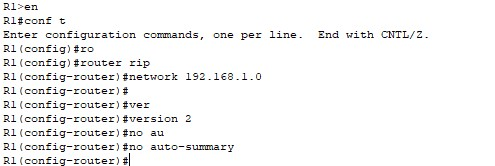
\includegraphics[width=0.75\textwidth]{8}
        \caption{Подключение протокола rip}
        \label{fig:image1}
    \end{figure}

    \begin{figure}[H]
        \centering      %размер рисунка       здесь находится название файла рисунка, без указания формата
        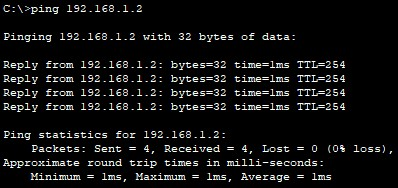
\includegraphics[width=0.75\textwidth]{9}
        \caption{Проверка доступности с компьютера администратора последовательного порта Маршрутизатора_2}
        \label{fig:image1}
    \end{figure}

    \item Проверьте доступность с компьютера администратора компьютеров в отделах проектирования.
    
    \begin{figure}[H]
        \centering      %размер рисунка       здесь находится название файла рисунка, без указания формата
        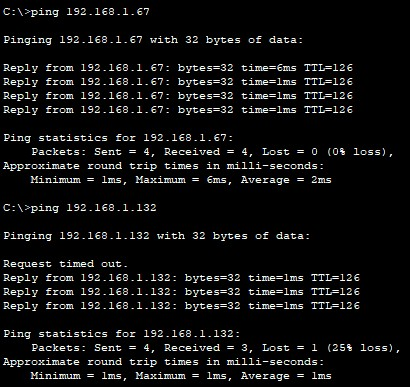
\includegraphics[width=0.75\textwidth]{10}
        \caption{Проверка доступности с компьютера администратора компьютеров в отделах проектирования}
        \label{fig:image1}
    \end{figure}
    
    \item Выполните ping с одного из компьютеров отдела проектирования интерьеров на любой из компьютеров в отделе проектирования зданий и сооружений.
    
    \begin{figure}[H]
        \centering      %размер рисунка       здесь находится название файла рисунка, без указания формата
        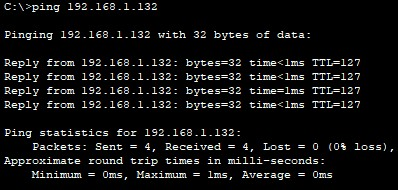
\includegraphics[width=0.75\textwidth]{7}
        \caption{Проверка доступности с компьютера отдела проектирования интерьера из компьютера из отдела проектирования зданий и сооружений}
        \label{fig:image1}
    \end{figure}

    \item Выполните ping с одного из компьютеров отдела проектирования интерьеров на любой из компьютеров в финансовом отделе.
    
    \begin{figure}[H]
        \centering      %размер рисунка       здесь находится название файла рисунка, без указания формата
        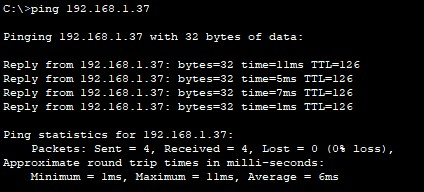
\includegraphics[width=0.75\textwidth]{11}
        \caption{Проверка доступности с компьютера отдела проектирования интерьеров компьютера в финансовом отделе}
        \label{fig:image1}
    \end{figure}

    \item Изучите таблицы маршрутизации на Маршрутизаторе_1 и Маршрутизаторе_2 и объясните полученные результаты.
    
    \begin{figure}[H]
        \centering      %размер рисунка       здесь находится название файла рисунка, без указания формата
        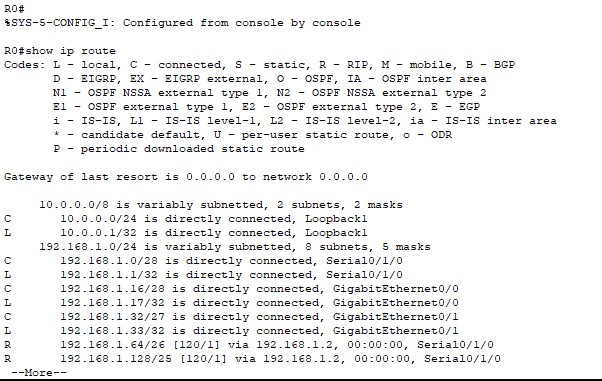
\includegraphics[width=0.75\textwidth]{13}
        \caption{Таблица маршрутизации первого роутера}
        \label{fig:image1}
    \end{figure}

    \begin{figure}[H]
        \centering      %размер рисунка       здесь находится название файла рисунка, без указания формата
        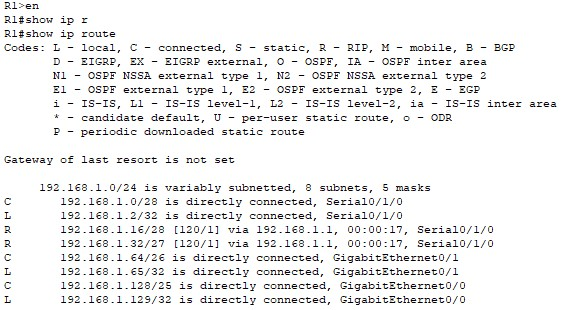
\includegraphics[width=0.75\textwidth]{12}
        \caption{Таблица маршрутизации второго роутера}
        \label{fig:image1}
    \end{figure}

    Изучив таблицы маршрутизации, мы видим, что роутеры подключены друг к другу через интерфейс Serial 0/1/0,
    а так же то, что через свои интерфейсы GigabitEthernet 0/0 и GigabitEthernet 0/1 каждый роутер подключен к двум.
    из четырех подсетей.

    \item Включите на маршрутизаторах вторую версию протокола RIP
    
    Данная версия протокола уже была подключена ранее.

    \item Просмотрите таблицы маршрутизации, зафиксируйте и объясните изменения
    
    Явно видимых изменений не наблюдается.

    \item На Маршрутизаторе_1 включите редистрибуцию статических маршрутов. Какие изменения после этого произошли в таблицах маршрутизации?
    
    \begin{figure}[H]
        \centering      %размер рисунка       здесь находится название файла рисунка, без указания формата
        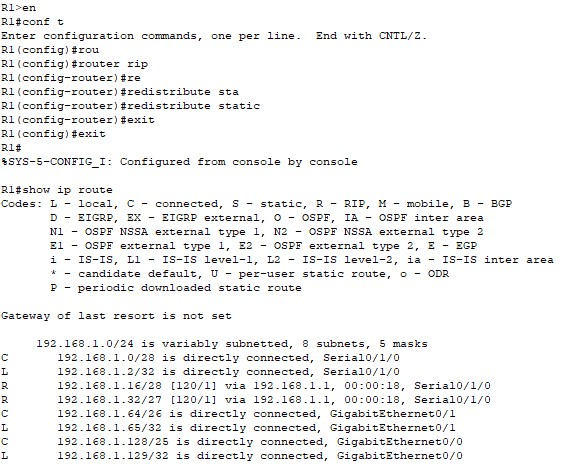
\includegraphics[width=0.75\textwidth]{14}
        \caption{Пример включения редистрибуции статических маршруов на роутере 2}
        \label{fig:image1}
    \end{figure}

    Явные изменения были не установленны.

    \item Убедитесь, что с любого из компьютеров сети можно выполнить ping на любой компьютер в любой подсети и на любое сетевое устройство. 
    
    Проверка прошла успешно.

    \item Сохраните сделанные изменения в конфигурациях

\end{enumerate}

\end{document}
